\documentclass{beamer}
% \usepackage[utf8]{inputenc}
\usepackage[utf8]{vietnam}
% \usepackage{xeCJK}
\usepackage{graphicx}
\usepackage {mathtools}
\usepackage{utopia} %font utopia imported
% \usetheme{Madrid}
% \usecolortheme{lily}
\usetheme{CambridgeUS}
\usecolortheme{dolphin}

% set colors
% \definecolor{myNewColorA}{RGB}{126,12,110}
% \definecolor{myNewColorB}{RGB}{165,85,154}
% \definecolor{myNewColorC}{RGB}{203,158,197}
% \setbeamercolor*{palette primary}{bg=myNewColorC}
% \setbeamercolor*{palette secondary}{bg=myNewColorB, fg = white}
% \setbeamercolor*{palette tertiary}{bg=myNewColorA, fg = white}
% \setbeamercolor*{titlelike}{fg=myNewColorA}
% \setbeamercolor*{title}{bg=myNewColorA, fg = white}
% \setbeamercolor*{item}{fg=myNewColorA}
% \setbeamercolor*{caption name}{fg=myNewColorA}
\usefonttheme{professionalfonts}
\usepackage{natbib}
\usepackage{hyperref}
%------------------------------------------------------------
% \titlegraphic{\includegraphics[eight=1.5cm]{figures/CityULogo.pdf}}

\setbeamerfont{title}{size=\large}
\setbeamerfont{subtitle}{size=\small}
\setbeamerfont{author}{size=\small}
\setbeamerfont{date}{size=\small}
\setbeamerfont{institute}{size=\small}
\title[Semantic version]{Semantic Version}
\subtitle{Quản lý project và gitflow theo semantic version}
\author[minhnt@nal.vn]{Nguyễn Thế Minh}

% \institute[minhnt@my.hust.edu.vn]{ Hà Nội University of Science and Technology}
\date[March 2025]{March 2025}

%------------------------------------------------------------
%This block of commands puts the table of contents at the
%beginning of each section and highlights the current section:
\AtBeginSection[]
{
 \begin{frame}
   \frametitle{Nội dung}
   \tableofcontents[currentsection]
 \end{frame}
}
% \AtBeginSection[]{
%   \begin{frame}
%   \vfill
%   \centering
%   \begin{beamercolorbox}[sep=8pt,center,shadow=true,rounded=true]{title}
%     \usebeamerfont{title}\insertsectionhead\par%
%   \end{beamercolorbox}
%   \vfill
%   \end{frame}
% }
%------------------------------------------------------------

\begin{document}

%The next statement creates the title page.
\frame{\titlepage}
\begin{frame}
\frametitle{Nội dung}
\tableofcontents
\end{frame}
%------------------------------------------------------------

%=========================
\section{Semantic version}
\begin{frame}
\frametitle{Mô hình quản lý semantic version}
\begin{itemize}
\item Source code và tài liệu của dự án được gán nhãn gọi là \textbf{semantic version} number.
\item Một semantic version được cấu tạo bởi 3 con số \textbf{major.minor.patch}
    \begin{itemize}
    \item Lần phát hành đầu tiên: \textit{1.0.0}
    \item \textbf{Patch release}: \textit{backward compatible} bug fixes, tăng patch, \textit{1.0.1}
    \item \textbf{Minor release}: \textit{backward compatible} new features, tăng minor và reset patch về 0, \textit{1.1.0}
    \item \textbf{Major release}: \textit{break backward compatibility}, tăng major, reset minor và patch về 0, \textit{2.0.0}
    \end{itemize}
\end{itemize}
\begin{definition}
\textbf{Backward compatible}: nghĩa là thay đổi nhưng không phá vỡ tính tương thích của sản phẩm như API, Interface,...
\end{definition}
\end{frame}

\begin{frame}
\frametitle{Git flow cho semantic version}
Với mỗi version, một branch code (\textbf{feature/1.1.0}, \textbf{feature/1.2.0}) tách ra từ nhánh chính (\textbf{develop}).
\begin{figure}[h!]
  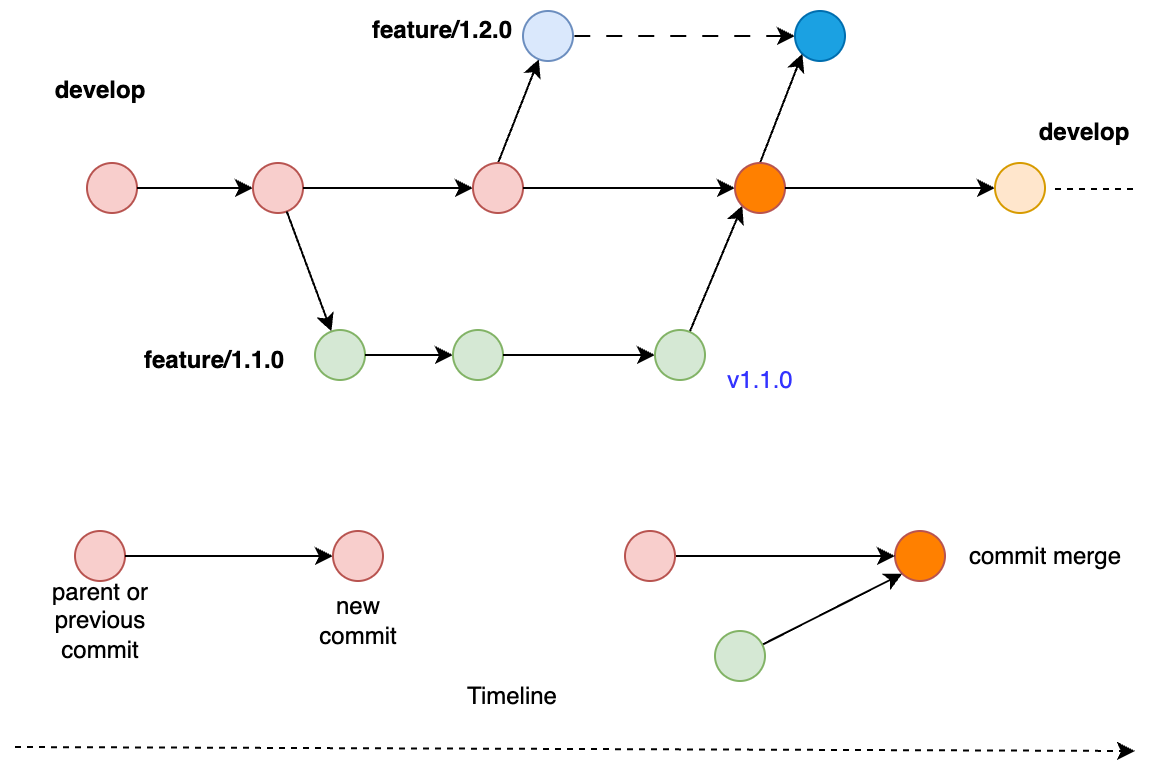
\includegraphics[height=7cm]{git-flow-overview.png}
\end{figure}
\end{frame}

\begin{frame}
\frametitle{Môi trường test}
Mỗi project sẽ có các môi trường test sau:
\begin{itemize}
\item \textbf{dev env}: đội dev NAL thực hiện test các chức năng (tickets) trong một version.
\item \textbf{uat env}: SYSTEM thực hiện test UAT cho một version.
\item \textbf{stg env}: SYSTEM thực hiện test staging cho một version trước khi release production.
\end{itemize}
\end{frame}

%===================
\section{Git flow cho minor version}
    \begin{frame}{Conclusion}
    \end{frame}

%===================
\section{Git flow cho patch fix}
    \begin{frame}{Conclusion}
    \end{frame}

%===================
\section{Git flow cho hotfix}
    \begin{frame}{Conclusion}
    \end{frame}

\section*{Acknowledgement}
\begin{frame}
% \textcolor{myNewColorA}{\Huge{\centerline{Thank you!}}}
\Huge{\centerline{Thank you!}}
\end{frame}

\end{document}
